\documentclass[11pt,a4paper]{article}

% Encodage et polices
\usepackage[utf8]{inputenc}
\usepackage[T1]{fontenc}
\usepackage{textcomp}
\usepackage{lmodern, microtype}

% Langue et géométrie (gardé 2.5cm, modifiable selon vos besoins)
\usepackage[english, french]{babel} 
\usepackage[margin=2.5cm]{geometry}

% Graphiques et tableaux
\usepackage{graphicx}
\graphicspath{{images/}}
\usepackage{booktabs}
\usepackage{tabularx}
\usepackage{longtable}
\usepackage{array}
\usepackage[table]{xcolor}

% Mise en page et outils
\usepackage{enumitem}
\usepackage{amsmath}
\usepackage{calc}
\usepackage{float}
\usepackage{siunitx}
\sisetup{locale=FR}
\usepackage{needspace}
\usepackage{pdfpages}
\usepackage{csquotes}

% TikZ
\usepackage{tikz}
\usetikzlibrary{arrows.meta, positioning}

% Bibliographie (biblatex)
\usepackage[backend=biber, style=numeric, sorting=none]{biblatex}
\addbibresource{refs.bib}

% Hyperliens (toujours charger en dernier, sauf si spécifié par la doc d'un package)
\usepackage[hidelinks]{hyperref}


\setlength{\tabcolsep}{4pt}
\renewcommand{\arraystretch}{1.3}
\setlength{\parindent}{0pt}
\setlist{itemsep=2pt,topsep=3pt}

% Placeholder for information still to be filled in
\newcommand{\todo}[1]{\textbf{[TO DO: #1]}}

\newcommand{\risqueentete}{%
  \toprule
  \textbf{Risk} & \textbf{Cause} & \textbf{Consequence} & \textbf{Level} & \textbf{Prevention} \\
  \midrule
  \endfirsthead
  \toprule
  \textbf{Risk} & \textbf{Cause} & \textbf{Consequence} & \textbf{Level} & \textbf{Prevention} \\
  \midrule
  \endhead
  \bottomrule
  \endfoot
}

\begin{document}

\begin{center}
{\Large \textbf{ARGUS Project}}\\[0.3em]
{\large Mission Definition, Payload Description}\\[0.5em]
ARGUS project -- November 2026
\end{center}

\small
\tableofcontents
\normalsize

% ==================================================================
\section{Mission Definition}
Our project named ARGUS for Autonomous Ranging Guidance for Uncontrolled Spacecraft, consists of a space debris deorbiting system using a \mot{6U} CubeSat, whose payload is made up of a \mot{LiDAR} a power  \mot{LASER} and a\mot{camera}. Its main motivation is to contribute to the space debris problem.\\
In the remainder of this document, we will endeavour to describe the whole payload \mot{LiDAR + LASER and camera} subsystem as exhaustively as possible, detailing the choice of each of its components. This approach will give us a clear and overall view of the direction to follow, while allowing us to stay within our budget forecasts.

\subsection{Studied object / functional mission target}
\textbf{Definitive choice:} space debris in low Earth orbit, a small object (about  less than 1\,kg, aluminium surface) to be tracked and deflected by a CubeSat.\\

%\newpage
\subsection{The LASER: \textbf{Light Amplification by Stimulated Emission of Radiation}}
In $1917$, Albert Einstein introduced the concepts of \textbf{absorption}, \textbf{spontaneous emission} and \textbf{stimulated emission} \cite{Einstein1917}. This was the beginning of LASER applications in industry and in the field of scientific research. \\
A laser is an optical device that makes it possible to amplify or produce radiation at frequencies in the \textbf{UV}, \textbf{infrared} or \textbf{visible} domains of the electromagnetic spectrum \cite{Siegman1986, Maiman1960}.\\
Laser sources have three main characteristics:
\begin{itemize}
    \item \textbf{Spatio-temporal coherence:} 
    Indeed, this characteristic of lasers allows us to know exactly over what temporal or spatial scale the phase information of one or several waves can be preserved.\\
    \item \textbf{Remarkable directivity:} 
    Unlike a mercury lamp, for example, whose photons are scattered in different directions, the laser has the particularity of being very weakly divergent and therefore carries the energy of the photons in a given direction.\\
    \item \textbf{A single colour:} 
    A laser is said to be monochromatic because its light radiation consists of a single wavelength. In fact, lasers are not totally monochromatic. It is possible to vary their wavelength: they are said to be tunable. For example, laser diodes make it possible to vary the wavelength of the Titanium-Sapphire (Ti:Sa) laser by typically $\Delta\lambda = 10nm$ \cite{Moulton1986}.
\end{itemize}
%\clearpage
\begin{figure}[H]
  \centering
  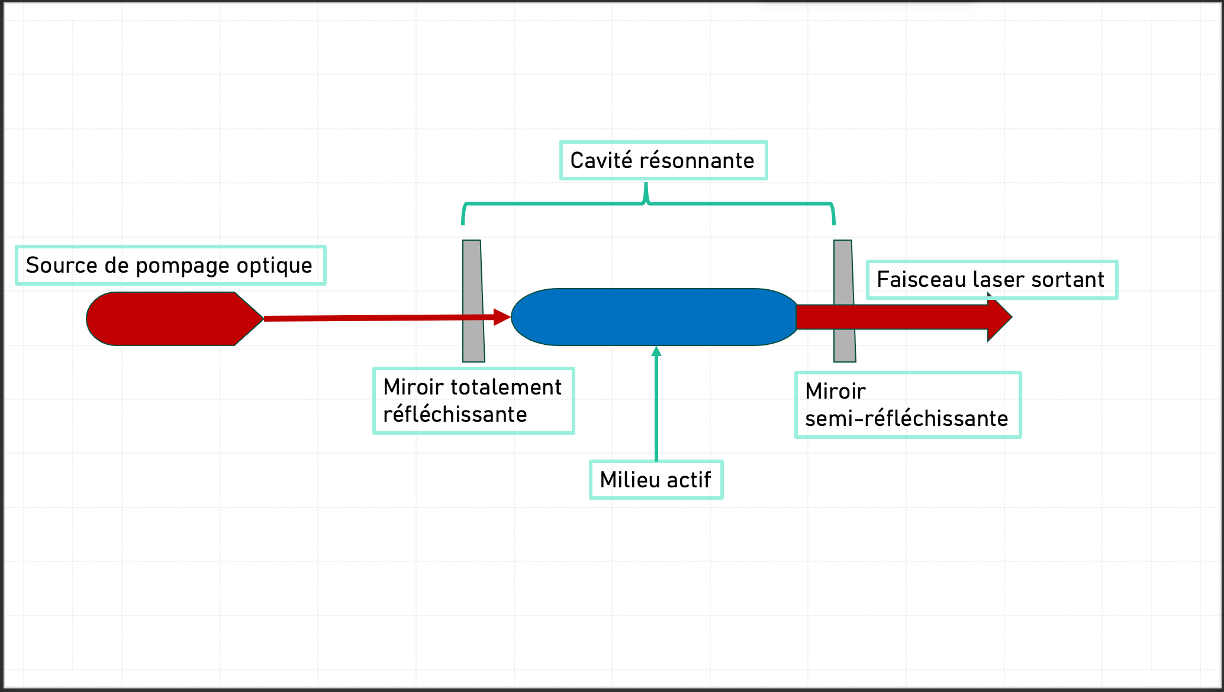
\includegraphics[width=0.8\textwidth]{image.png}
  \caption{Illustration of the operating principle of a laser}
  \label{fig:argus}
\end{figure}

\subsection{The LiDAR: Light Detection and Ranging}
The LiDAR is an active remote-sensing tool that makes it possible to measure certain atmospheric parameters (\textbf{$\rho$}, \textbf{wind}, \textbf{T}, \textbf{P}) and constituents ( \textbf{$H_{2}O$}, \textbf{$O_{3}$}...).\\
The physical principle of a Lidar consists in emitting a light beam that will interact, in all directions, with the medium in which it propagates. The radiation returning toward the instrument by backscattering is then detected.\\
\begin{figure}[H]
  \centering
  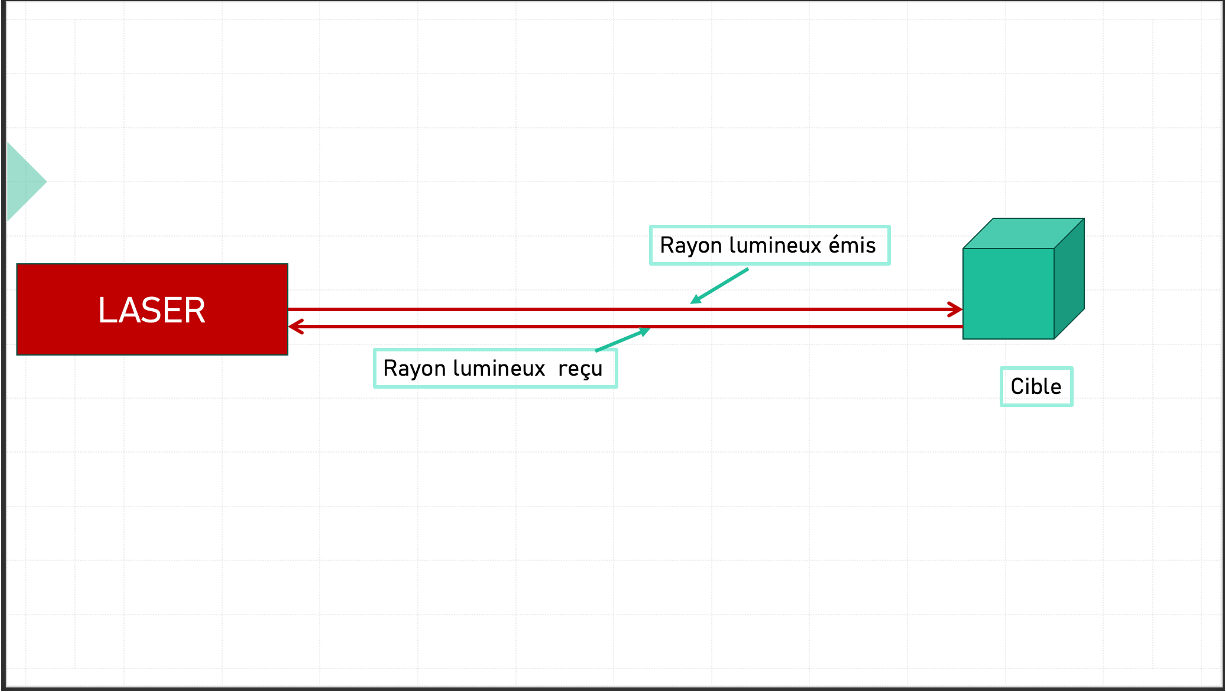
\includegraphics[width=0.8\textwidth]{Lidar_.png}
  \caption{Operating principle of a LiDAR}
\end{figure}

The expression used to calculate the round-trip distance of the laser beam is given by: 
\begin{equation}
    \boxed{\mathbf{Distance = \frac{c * t}{2}}}
\end{equation} 
with \textbf{c} the speed of light and \textbf{t} the travel time of the light.


\section{Scientific / technological question or aim}
\textbf{Definitive choice:} demonstrate that a 6U CubeSat can detect and track a small debris at short range with a LiDAR, and change its trajectory by laser ablation (target : small $\Delta V$).
\\

%\newpage
\subsection{The debris}
For the laser ablation process to work effectively without fragmenting the debris, which would feed the \textbf{Kessler syndrome} \cite{Kessler1978}, the material must efficiently absorb the wavelength of our high-power laser (which we will define in the infrared). We choose an aluminium (Al) debris, a material that is very common in space structures \cite{Graham2001}. Mechanical coupling there is maximal for LASER intensities of the order of \SI{e9}{\watt\per\centi\metre\squared} at the transition between the vapour and plasma regimes \cite{Jin2013}. \\
Table \ref{tab:debris_al} summarizes the characteristics of the aluminium retained for the ARGUS mission.
\Needspace{7cm}
\begin{table}[H]
  \centering
  \caption{Characteristics of the aluminium used as debris \cite{Phipps2012}.} 
  \label{tab:debris_al}
  \begin{tabular}{p{6cm} p{6cm}}
    \toprule
    \textbf{Characteristic} & \textbf{Value} \\
    \midrule
    Type of aluminium & [Space alloys of type 7075 or 6061] \\
    Thickness & [\SI{1}{\centi\metre}] to [\SI{10}{\centi\metre}] \\
    Target surface & [\SI{0.03}{\centi\metre\squared}] \\
    Density of aluminium & \SI{2700}{\kilo\gram\per\metre\cubed} \\
    Debris mass & [\SI{1}{\kilo\gram}] \\
    Ablation threshold of aluminium & [\SI{2}{\joule\per\centi\metre\squared}] \\
    \bottomrule
  \end{tabular}
\end{table}


%\newpage
\subsection{The choice of the launch orbit}
Our $6U$ CubeSat will be placed in low Earth orbit (LEO, \textit{Low Earth Orbit}) at an altitude between \SIrange{200}{600}{\kilo\metre}. The lower limit is set by atmospheric drag, above the \textbf{Karman line}, the conventional boundary of space located at about \SI{100}{\kilo\metre} altitude \cite{McDowell2018}. Three main reasons motivate this choice:
\begin{itemize}
    \item The energy limit imposed on us by the size of a $6U$.\\

    \item The urgency of cleaning up the LEO orbit. LEO is the most densely populated region of space in terms of debris, because of decades of space activities and the development of mega-constellations such as Starlink. ESA estimates the number of debris objects larger than $1 cm$ at more than $1.2$ million, of which more than $50000$ exceed $10cm$\cite{ESA2025}. Debris of \SIrange{1}{10}{\centi\metre} travels there at about $7.5 Km/s$\cite{Vallado2013}. Testing our laser-ablation deorbiting system (ARGUS) in LEO thus meets one of the most urgent needs of the space industry.
    %The urgency of cleaning up the LEO orbit. LEO is the most densely populated region of space in terms of debris, because of decades of space activities and the development of mega-constellations such as Starlink. ESA estimates the number of debris objects larger than $1 cm$ at more than $1.2$ million, of which more than $50000$ exceed $10 cm$ \cite{ESA2025}. Debris of \SIrange{1}{10}{\centi\metre} travels there at about \SIrange{7.5}{\kilo\metre\per\second} \cite{Vallado2013}. Testing our laser-ablation deorbiting system (ARGUS) in LEO thus meets one of the most urgent needs of the space industry.

    \item Our ablation device lowers the perigee of the debris in order to bring it closer to the dense layers of the atmosphere \cite{Phipps2012}, where drag accelerates its disintegration. Depending on the altitude, reentry can occur after a few days, a few months or a few years \cite{Crisp2020}. 
\end{itemize}
\begin{table}[H]
  \centering
  \small
  \caption{Summary of the advantages of low Earth orbit (LEO) for the project.}
  \label{tab:leo}
  \begin{tabular}{p{3.5cm} p{5.5cm} p{5.5cm}}
    \toprule
    \textbf{Mission parameter} & \textbf{Advantage in LEO (200--600 km)} & \textbf{Risk on another orbit (e.g. MEO/GEO)} \\
    \midrule
    Launcher availability & Monthly rideshare flights & Very rare and custom-made for CubeSats \\
    Safety of the released debris & Fast natural disintegration in case of failure & The debris becomes permanent pollution \\
    LIDAR/laser link budget & Short, manageable distance & Would require megawatt-class lasers \\
    Project cost & Suited to academic budgets & Multiplied by 5 to 10 \\
    \bottomrule
  \end{tabular}
\end{table}


\subsection{The operational scenario}
In theory, the different phases of the ARGUS mission should unfold chronologically as follows: 
\begin{enumerate}
    \item \textbf{Transport and orbit insertion:}
    Our debris must be firmly secured to our chaser CubeSat from launch until orbit insertion. \\
    
    \item \textbf{Release: }
    A mechatronic mechanism must allow us to eject our debris at a relatively very low speed (about \SIrange{0.1}{0.5}{\metre\per\second}) so that it moves away slowly without a dangerous trajectory. These values are significantly lower than the \SIrange{1}{3}{\metre\per\second} of conventional CubeSat deployers \cite{CSD_AFIT} in order to limit the relative drift after separation \cite{FormationRelease}. \\
    
    \item \textbf{Detection:}
    As soon as the debris is released, the LiDAR detects and tracks it. At a relatively short distance ( \SIrange{10}{100}{\metre\per\second}), it provides the position of the debris in real time with a precision of the order of a centimetre, which can reach the millimetre after averaging several pulses \cite{DLR2014} and \cite{Vela2022}.\\
    
    \item \textbf{LASER firing:} 
    Once the debris is at a safe distance and perfectly aligned, the high-power LASER performs scheduled shots opposite to the debris's velocity vector to slow it down and lower its perigee into the atmosphere. \cite{Phipps2012}.\\
    
    \item \textbf{Deorbiting and atmospheric disintegration: }
    Once its perigee has been lowered, the debris gets closer to the dense atmosphere. This leads to atmospheric entry followed by faster disintegration due to the influence of atmospheric drag \cite{Bekey1997}. 
\end{enumerate}
%\clearpage
\begin{figure}[H]
  \centering
 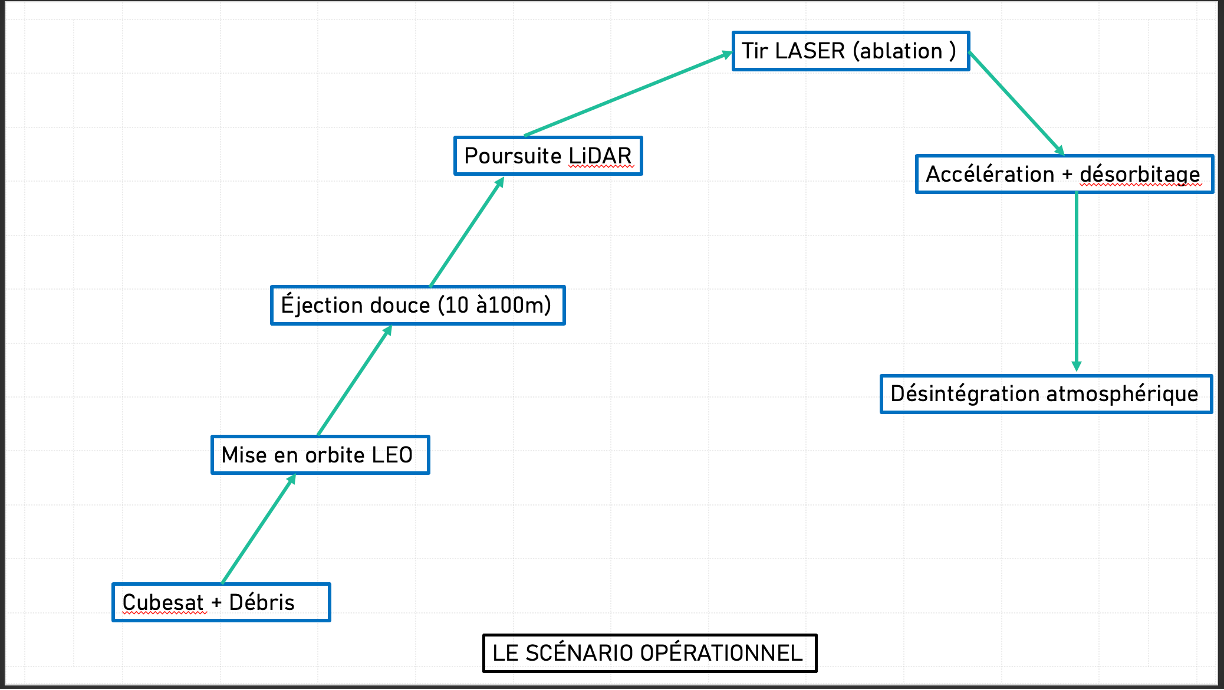
\includegraphics[width=0.8\textwidth,height=7cm,keepaspectratio]{chrono_argus.png}
  \caption{Illustration of the chronological stages of the ARGUS mission}
  \label{fig:laser}
\end{figure}

%\subsection{Main payload}
%The main payload of the Argus mission is the debris, which we aim to eject.
%The shape of the debris has not been finalized, but it will be a small object weighing less than 1\,kg with an aluminium surface.
%The second main payload is the laser, a Class 4 laser with a wavelength of 1064\,nm.

%\subsection{Secondary payloads}
%The laser will be guided by a LiDAR (secondary payload) operating at a wavelength of 1550\,nm, equipped with a SPAD detector and a MEMS micro-mirror.
%The second secondary payload is a camera with a machine learning algorithm to detect the debris and estimate its orientation.
%Thanks to these two instruments, we can track the debris and fire the laser at it.
\newpage
\subsection{Experts contacted}
%Vincent robert, teacher at ipsa about space mechanics. He can have a look at the feasibility of the mission. But he don't have to much time to discute and help us.\\

% Required packages (already used in your document): booktabs, float
% \usepackage{booktabs}
% \usepackage{float}


% Packages nécessaires :
% \usepackage{booktabs}
% \usepackage{float}
% \usepackage{needspace}
% \usepackage{array}

\Needspace{8cm}
\begin{table}[H]
  \centering
  \footnotesize
  \caption{Experts contacted during the ARGUS project.}
  \label{tab:experts}
  \begin{tabular}{
    p{2.8cm}
    p{3.2cm}
    p{3.0cm}
    p{2.3cm}
    p{3.4cm}
  }
    \toprule
    \textbf{Name and position} &
    \textbf{Organisation} &
    \textbf{Area of expertise} &
    \textbf{Date and contact method} &
    \textbf{Key input provided} \\
    \midrule

    Pr. Philippe KECKHUT,
    Directeur de l'académie spatial d'ile-de-France
    &
    Université Paris Saclay, 
    UVSQ, France
    &
    LiDAR technology and optical detection
    &
    05/11/2026, 
    Philippe.Keckhut@
    latmos.ipsl.fr
    &
    Recommendations on LiDAR use and the optical system set up.\\

    \addlinespace

    Vincent ROBERT,
    Mechanic Systems Engineer,
    Professor at IPSA
    &
    IPSA, France
    &
    LiDAR technology and optical detection
    &
    06/11/2026, video call
    &
    Advice on LiDAR architecture, signal acquisition and detection performance. \\

    \addlinespace

    %Julien Bernard,
    %Space Systems Engineer
    &
    %Airbus Defence and Space, France
    &
    %Small satellite and CubeSat engineering
    &
    %09/11/2026, meeting
    &
    %Guidance on payload integration, platform constraints and system-level design. \\

    \addlinespace

    %Sophie Laurent,
    %Space Safety Specialist
    &
    %CNES, France
    &
   % Space debris mitigation and mission safety
    &
    %10/11/2026, email
    &
    %Information on orbital safety, debris mitigation and end-of-life requirements. \\

    \addlinespace

    %Antoine Moreau,
    %Orbital Mechanics Engineer
    &
    %ArianeGroup, France
    &
    %Orbital mechanics and mission analysis
    &
   % 12/11/2026, phone call
    &
    %Advice on orbital parameters, mission constraints and trajectory considerations. \\

    \bottomrule
  \end{tabular}
\end{table}


% ==================================================================
\section{Payload Description}
% ---------- Payload ----------

Sizing a LASER-ablation deorbiting system involves a direct physical trade-off:
 the LASER must not destroy the debris through excessive heat input, 
 but must vaporise a very thin layer of its surface to create a propulsive plasma that slows the moving debris. 
 Thus, modifying the orbit of an object (debris) relies on converting the optical energy deposited by laser pulses into the mechanical energy of the plasma jet.

\subsection{LASER Ablation Propulsion}
When a high-intensity LASER beam strikes the surface of a material, 
the optical energy is absorbed instantaneously. 
The temperature of the surface layer rises so rapidly that it undergoes sudden sublimation and becomes a highly energetic plasma. 
This jet of matter is expelled at very high speeds. Under the physical law of conservation of matter, the ejection of matter generates a mechanical recoil force on the target object \cite{Vincent2011}.

\begin{figure}[H]
  \centering
  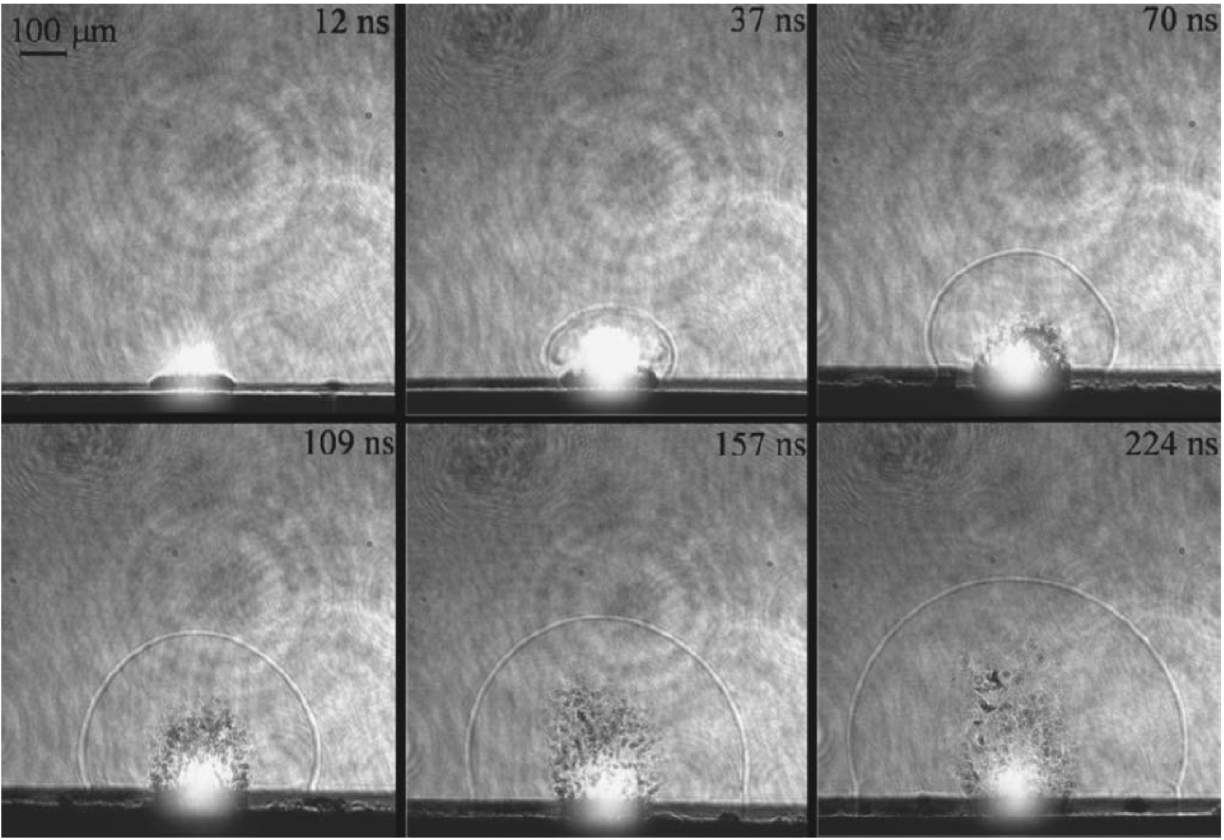
\includegraphics[width=0.8\textwidth,height=7cm,keepaspectratio]{ablation_laser.png}
  \caption{Images of the ablation propulsion process at different times during the laser--aluminium interaction for $\lambda = 1064 nm$ and $\tau = 5ns$. The propagation of the shock wave over time can be observed. \cite{Vincent2011}}
  \label{fig:ablation}
\end{figure}

\subsection{High-Power LASER Characteristics}
In this section, we describe the characteristics of our onboard high-power LASER. 
Selecting the high-power LASER is crucial: if its power or energy is unsuitable, 
it will probably not be possible to initiate the micropropulsion process at the surface of our target (debris).

\begin{enumerate}
    \item \textbf{Choice of LASER type:}\\
    We choose a pulsed LASER rather than a continuous-wave laser. 
    The factors determining this choice are summarised in the table below

    \begin{table}[H]
      \centering
      \caption{Comparison between continuous-wave and pulsed lasers.}
      \begin{tabular}{p{3.5cm} p{5.5cm} p{5.5cm}}
        \toprule
        \textbf{Characteristic} & \textbf{Continuous-wave laser } & \textbf{Pulsed laser} \\
        \midrule
        Effect on debris & Thermal melting  & Plasma ablation (mechanical rocket effect) \\
        Peak power & Equal to average power  & Several megawatts during the pulse \\
        Generated thrust & Almost zero at this power level & Optimal and directional \\
        Risks & High risk of breaking up the debris & Safe, targeted surface action \\
        \bottomrule
      \end{tabular}
    \end{table}

    \item \textbf{Required LASER parameters:}\\
    The wavelength of our high-power LASER is set to $\lambda = $\SI{1064}{\nano\metre} in the infrared, with a pulse duration of \textbf{nanoseconds (ns)}. This choice is primarily based on the absorption characteristics of the material making up our debris, namely aluminium (Al).

    For this CubeSat project using a $6U$ platform firing a LASER at short range, the optimal average power required for our small aluminium debris object, measuring \SIrange{1}{10}{\centi\metre} and weighing $1kg$ is approximately $1000W$. The choice of this operating power is deliberate and results from a specific trade-off validated by orbital mechanics and the physics of laser--matter interaction. The section on project feasibility discusses in detail the importance of reaching this optimal LASER ablation power.

    \begin{table}[H]
      \centering
      \small
      \caption{Ablation laser parameters.}
      \label{tab:laser_ablation}
      \begin{tabular}{p{6cm} p{6cm}}
        \toprule
        \textbf{Parameter} & \textbf{Value} \\
        \midrule
        Wavelength ($\lambda$) & \SI{1064}{\nano\metre} (infrared) \\
        Operating mode & Pulsed \\
        Pulse duration ($\tau$) & Nanosecond (ns) \\
        Average power ($P_{\text{moy}}$) & \SI{1000}{\watt} (\SI{1}{\kilo\watt}) \\
        Repetition rate ($f$) & \SI{3000}{\hertz} (\SI{2}{\kilo\hertz}) \\
        Pulse energy ($E_p$) & \SI{0.5}{\joule} \\
        Peak power ($P_{\text{crête}}$) & \SI{100}{\mega\watt} \\
        Ablation threshold fluence & \SIrange{1}{2}{\joule\per\centi\metre\squared} \\
        Optimal coupling fluence & \SI{5}{\joule\per\centi\metre\squared} \\
        \bottomrule
      \end{tabular}
    \end{table}
\end{enumerate}

%\newpage
\subsection{LiDAR for Detection}
To meet the imposed dimensional constraints, we favour a micro-LiDAR over a conventional LiDAR, which would entail higher mass and energy demands. The micro-LiDAR provides optical metrology of the debris: detection, relative position and relative velocity \cite{OpromollaNocerino}. It consists of three main elements:
\begin{itemize}
    \item The emission source, which in our case could be a VCSEL (Vertical Cavity Surface Emitting LASER). These are arrays of miniature semiconductor LASERs. The table below summarises the parameters we consider optimal for defining the LASER source of our micro-LiDAR.

    \begin{table}[H]
      \centering
      \small
      \caption{Micro-LiDAR laser parameters \cite{VCSEL1550_2023}.}
      \label{tab:lidar_laser}
      \begin{tabular}{p{3.3cm} p{4.7cm} p{6.5cm}}
        \toprule
        \textbf{Parameter} & \textbf{Specified value} & \textbf{Purpose in space} \\
        \midrule
        Wavelength & \SI{1550}{\nano\metre} & Prevents blinding by the ablation laser (\SI{1064}{\nano\metre}) \\
        Source type & Pulsed laser diode (InGaAs) & Robustness, extreme compactness \\
        Pulse duration & \SI{3}{\nano\second} & Millimetre-level ranging accuracy \\
        Frequency & \SI{20}{\kilo\hertz} & Smooth real-time target tracking \\
        Pulse energy & \SI{10}{\micro\joule} & Completely harmless to the debris \\
        Electrical power consumption & $\approx\SI{12}{\watt}$ & Fully suited to the constraints of a 6U CubeSat \\
        \bottomrule
      \end{tabular}
    \end{table}

    \item An ultrasensitive SPAD (Single Photon Avalanche Diode) detector. These detectors can detect a single returning photon. The table below summarises the parameters we consider optimal for selecting a suitable detector for our micro-LiDAR \cite{Pellegrini2006}.

    \begin{table}[H]
      \centering
      \small
      \caption{Micro-LiDAR SPAD detector parameters \cite{SPADReview2024}.}
      \label{tab:lidar_spad}
      \begin{tabular}{p{3.3cm} p{4.7cm} p{6.5cm}}
        \toprule
        \textbf{Parameter} & \textbf{Specified value} & \textbf{Purpose in space} \\
        \midrule
        Detector type & SPAD InGaAs/InP & Sensitive at \SI{1550}{\nano\metre}, single-photon detection \\ % to be verified
        Detection efficiency & $\approx\SI{20}{\percent}$ at \SI{1550}{\nano\metre} & Detect the weak signal backscattered by the debris \\ % to be verified
        Timing jitter (\textit{jitter}) & $\approx\SI{200}{\pico\second}$ & Range resolution of a few centimetres \\ % to be verified
        Dark count rate & $\approx\SI{10}{\kilo\hertz}$ (cooled detector) & Limit noise to maintain a good signal-to-noise ratio \\ % to be verified
        Operating mode & Gated (\textit{gated}), synchronised with the pulse & Reduce noise and power consumption \\ % to be verified
        \bottomrule
      \end{tabular}
    \end{table}

    \item MEMS (Micro-Electro-Mecanical System) micromirrors. These oscillating micromirrors are etched into silicon to steer the beam without heavy mechanical components. The table below summarises the parameters we consider optimal for selecting the mirror assembly for our micro-LiDAR \cite{Shea2006}.

    \begin{table}[H]
      \centering
      \small
      \caption{Micro-LiDAR oscillating MEMS micromirror parameters \cite{Liu2022}.}
      \label{tab:lidar_mems}
      \begin{tabular}{p{3.3cm} p{4.7cm} p{6.5cm}}
        \toprule
        \textbf{Parameter} & \textbf{Specified value} & \textbf{Purpose in space} \\
        \midrule
        Scanning mechanism & Resonant MEMS micromirror & Scene scanning without bulky mechanical components \\ % to be verified
        Mirror diameter & $\approx\SI{1}{\milli\metre}$ & Trade-off between optical aperture and resonant frequency \\ % to be verified
        Optical scan angle & $\pm\SI{10}{\degree}$ & Cover the field of view required for target acquisition \\ % to be verified
        Resonant frequency & $\approx\SI{1}{\kilo\hertz}$ & Scan rate compatible with real-time tracking \\ % to be verified
        Electrical power consumption & Less than $\SI{1}{\watt}$ & Compatible with the power budget of a 6U CubeSat \\ % to be verified
        \bottomrule
      \end{tabular}
    \end{table}
\end{itemize}


\subsection{Machine Learning and Computer Vision}\label{subsec:ml_cv}

\subsubsection{Functional description}
The Auricam D35 acquires monochrome images of the 1--10\,cm debris. A SpaceWire
interface on the Q8S carrier receives the images; the Q8S handles buffering,
calibrated image preprocessing and pose estimation, while the CogniSAT-XE2 runs
the neural networks over Ethernet. SSD-MobileNetV2 detects the debris during
initial acquisition and reacquisition. HRNet-W32 then locates 2D keypoints in a
region cropped from the native image, rather than from the reduced detector input.

SQPnP initializes the relative pose from calibrated 2D--3D correspondences with
a metric model of the debris. During tracking, an adaptive UKF combines the
keypoint measurements with the motion model to estimate relative position,
velocity, attitude and angular rate. Its predicted pose sets the next image
crop; unreliable points are rejected or down-weighted. The navigation output
contains a timestamp, state estimate, covariance and tracking-quality flags.
The camera, LiDAR and spacecraft attitude measurements require synchronized
timestamps and calibrated reference frames. Network training is performed on
the ground; fixed FP16 models are deployed in flight.

\subsubsection{Quantitative specifications}
\begin{table}[H]
\centering\small
\renewcommand{\arraystretch}{1.45}
\setlength{\tabcolsep}{6pt}
\caption{Auricam D35 camera configuration.}
\label{tab:ml_cv_camera}
\begin{tabularx}{\linewidth}{|>{\raggedright\arraybackslash}p{3.6cm}|>{\raggedright\arraybackslash}X|}
\hline
\rowcolor{black!8}
\textbf{Parameter} & \textbf{Specification / configuration} \\
\hline
Optics & 25\,mm focal length, $f/3.5$; $35^{\circ}$ diagonal field of view ($\approx25.4^{\circ}$ per side); $38^{\circ}$ solar exclusion angle \\
\hline
Sensor & Monochrome $2048\times2048$, $5.5\,\mu$m pixel pitch, global shutter; 12-bit native output \\
\hline
Frame rate & 2.5 frames/s at full resolution; 10 frames/s at $1024\times1024$ with $2\times2$ binning; 2\,Hz nominal mission acquisition \\
\hline
Exposure / timing & $60\,\mu$s--30\,s exposure; image timestamp accuracy $<1$\,ms \\
\hline
Camera interface & SpaceWire at 20/40/80/160\,Mbit/s; 160\,Mbit/s selected; regulated 5\,V supply (4.6--6\,V input range) \\
\hline
Mechanical / thermal & $80\times80\times140$\,mm with baffle; 420\,g; mounting-base temperature $-35$ to $+55\,^{\circ}$C \\
\hline
Focus / calibration & Focus setting to be validated over 2--10\,m; intrinsic parameters, distortion, mounting alignment and thermal stability calibrated on the assembled system \\
\hline
\end{tabularx}
\end{table}

\begin{table}[H]
\centering\small
\renewcommand{\arraystretch}{1.45}
\setlength{\tabcolsep}{6pt}
\caption{Onboard processing hardware and data interfaces.}
\label{tab:ml_cv_processing}
\begin{tabularx}{\linewidth}{|>{\raggedright\arraybackslash}p{3.6cm}|>{\raggedright\arraybackslash}X|}
\hline
\rowcolor{black!8}
\textbf{Element} & \textbf{Specification / task} \\
\hline
Xiphos Q8S & Zynq UltraScale+ XCZU7EG; 4$\times$ Cortex-A53, 2$\times$ Cortex-R5 and FPGA; 4\,GB LPDDR4 with EDAC; 2$\times$128\,GB eMMC. Image reception, ROI extraction, SQPnP, adaptive UKF and telemetry. \\
\hline
Q8S mechanical & $80\times80\times11.2$\,mm; 56\,g excluding connectors; watchdog and FPGA/memory error protection. \\
\hline
CogniSAT-XE2 & Myriad X vision accelerator; PC/104 format; approximately 80\,g. FP16 inference for SSD-MobileNetV2 and HRNet-W32; simultaneous graph residency to be verified. \\
\hline
Data paths & Auricam $\rightarrow$ Q8S carrier: SpaceWire with FPGA logic/transceivers; Q8S $\leftrightarrow$ XE2: Ethernet. Carrier supplies regulated rails, including 5\,V for the camera and XE2. \\
\hline
Software / buffering & Linux ARM64 host and compatible Ubotica/OpenVINO toolchain; initially 1\,GiB of Q8S RAM reserved for vision. One native frame uses 8\,MiB in a 16-bit RAM container. \\
\hline
\end{tabularx}
\end{table}

\begin{table}[H]
\centering\small
\renewcommand{\arraystretch}{1.45}
\setlength{\tabcolsep}{6pt}
\caption{Vision processing parameters and verification targets.}
\label{tab:ml_cv_performance}
\begin{tabularx}{\linewidth}{|>{\raggedright\arraybackslash}p{3.7cm}|>{\raggedright\arraybackslash}X|}
\hline
\rowcolor{black!8}
\textbf{Parameter} & \textbf{Value} \\
\hline
Detector & SSD-MobileNetV2; $320\times320$ input; bounding box and confidence score; invoked at acquisition, periodic checks and tracking loss. \\
\hline
Keypoint network & HRNet-W32; $256\times256$ native-image crop; 28.5 million parameters ($\approx57$\,MB FP16 weights); keypoints and confidence maps. \\
\hline
Pose / filter & SQPnP initialization from a metric 3D target model; UKF propagation at 20\,Hz and optical corrections at 2\,Hz. \\
\hline
Image link budget & At 2\,Hz: 12-bit packed full frames $\approx126$\,Mbit/s including SpaceWire character overhead; 16-bit unpacked frames $\approx168$\,Mbit/s and exceed the 160\,Mbit/s link. Packet overhead and pixel packing require interface verification. \\
\hline
Relative geometry & 1--10\,cm projected target dimension; 2--10\,m evaluation range. At 10\,m: $\approx4.5$--45.5 native pixels, or $\approx0.7$--7.1 pixels in a full frame resized to 320 pixels. \\
\hline
Accuracy target & Position error $\leq10$\,cm and attitude error $\leq3^{\circ}$ at the 95th percentile over the 2--10\,m test range. \\
\hline
Timing / deployment targets & Image-to-output age $<0.8$\,s (99th percentile, normal tracking); reacquisition $<5$\,s; $<10\%$ increase in the selected pose-error percentile after FP32-to-FP16 conversion. \\
\hline
Subsystem envelope & 1\,kg and 2U allocated, including camera, boards, carrier and harness; camera + Q8S + XE2 mass $\approx556$\,g before integration hardware. \\
\hline
\end{tabularx}
\end{table}

\begin{table}[H]
\centering\small
\renewcommand{\arraystretch}{1.45}
\setlength{\tabcolsep}{6pt}
\caption{Electrical power allocation for the vision subsystem.}
\label{tab:ml_cv_power}
\begin{tabularx}{\linewidth}{|>{\raggedright\arraybackslash}p{4.15cm}|>{\raggedright\arraybackslash}p{2.8cm}|>{\raggedright\arraybackslash}X|}
\hline
\rowcolor{black!8}
\textbf{Equipment} & \textbf{Documented power} & \textbf{Design allocation} \\
\hline
Auricam D35 camera head (without optional electronics unit) & 2\,W & 3\,W \\
\hline
CogniSAT-XE2 & 2.5\,W typical & 5\,W \\
\hline
Xiphos Q8S & 5\,W typical & 6\,W \\
\hline
Carrier and interfaces & Configuration-dependent & 1\,W \\
\hline
\rowcolor{black!4}
\textbf{Total equipment allocation} & & \textbf{15\,W} \\
\hline
\rowcolor{black!4}
\textbf{Satellite bus allocation} & & \textbf{22\,W} \\
\hline
\end{tabularx}
\end{table}

The 22\,W bus allocation includes 90\% conversion efficiency and a 30\%
sizing margin ($15/0.90\times1.30\approx21.7$\,W). All accuracy, latency and
power allocations require end-to-end verification on Auricam--Q8S--XE2 hardware.
At small apparent target sizes, detector resolution and pose observability
must also be validated; a restricted search window may be necessary.


%\subsection{Functional description of the payloads' behavior}
%%%\todo{complete and check the sequence below}
%\begin{enumerate}
%\item \textbf{Detection:} the LiDAR scans its field of view ($\pm 10^\circ$) and detects the debris.
%\item \textbf{Tracking:} the LiDAR measures the position of the debris and keeps tracking it; the fine pointing mirror is guided by the LiDAR data.
%\item \textbf{Lock check:} firing is authorized only if the target is locked (shutter opened).
%\item \textbf{Firing:} short laser bursts on battery power, ablating the aluminium surface to produce thrust.
%\item \textbf{Monitoring:} the debris is tracked during and after each burst; firing stops automatically in case of anomaly (fluence, loss of tracking).
%\item \textbf{Safe state:} firing inhibited by default outside the contact windows or without lock.
%\end{enumerate}

%\subsection{Quantified description of the payloads' performance}

%\todo{quantified performance table of all payloads -- to be discussed with the other subsystem}



\newpage
\section{Mission Feasibility}
This section aims to assess the feasibility of the ARGUS mission. To do so, we will need to calculate several key parameters that are essential for the successful execution of the mission. These calculations will also allow us to validate the various parametric choices related, in particular, to our selected LASER sources, the material composing our debris, and the choice of the target orbit.

\subsection{Theoretical Calculation Process for Selected LASER Parameters}

\begin{itemize}
    \item \textbf{Ablation threshold and optimal fluence (F)}\\
    The fluence of our LASER, with a wavelength of $\lambda = 1064 nm$ and \textbf{nanosecond (ns)} pulses, represents the energy delivered by this laser per unit area. It is expressed in \textbf{$J/cm^{2}$}. In the scientific literature, we find that the theoretical ablation threshold begins at approximately $F_{th} \approx 1 J/cm^{2}$ and can reach $F_{th} \approx 2 J/cm^{2}$ (reference to be added: Phipps). However, in our case, in order to achieve the optimal propulsive effect required, we need to reach the maximum coupling fluence $F_{couplage}$, defined by: \\
    \begin{equation}
    \boxed{F_{couplage} \approx  2.5 F_{th} \approx  5 J/cm^{2}}
    \end{equation}
    for $F_{th} = 2 J/cm^{2}$\\

    \item \textbf{Energy per pulse \textbf{$E_{P}$} and peak power \textbf{$P_{c}$}}\\
    The energy per pulse represents the total amount of energy contained in a single LASER pulse. It is calculated using the following formula:
    \begin{equation}
        \boxed{E_{P} = S *  F_{couplage} }
    \end{equation}
    $S$ represents the surface area impacted by the LASER pulse. For a focal spot diameter chosen as $d = 0.3 cm$, assuming a circular spot, we obtain the following value for $S$:
    \begin{equation}
      \boxed{  S = \frac{\pi d^{2}}{4} =\frac{\pi * (0.3)^{2}}{4} \approx 0.071 cm^{2} }
    \end{equation}
    Using this value of $S$, we finally obtain:
    \begin{equation}
        \boxed{E_{P} = 0.071 *5 = 0.35J }
    \end{equation}
    Thus, using this value of $E_{P}$, we can determine the instantaneous peak power \textbf{$P_{c}$} generated by our LASER. This power represents the energy flow per unit of time. Indeed, it is the maximum power reached by the LASER at the very core of the pulse. It is obtained by dividing the energy per pulse by the pulse duration.
    \begin{equation}
        \boxed{P_{c} = \frac{E_{P}}{\tau} = \frac{0.35}{5.10^{-9}} = 70MW}
    \end{equation}
    \\

    \item \textbf{Repetition frequency $f_{rep}$ and average power $P_{moy}$}\\
    To maintain the payload within a $6U$ CubeSat, we assume an average power of $P_{moy} = 1000 W$. This value is not arbitrary; it is mainly dictated by the thermal dissipation limit of a $6U$ CubeSat (reference to be added).\\
    Using this value, we calculate the pulse repetition frequency with the following formula: \\
    \begin{equation}
        \boxed{f_{rep} = \frac{P_{moy}}{E_{P}} = \frac{1000W}{0.35 J}  = 2857 Hz \approx 3KHz}
    \end{equation}

\end{itemize}

\subsection{Calculation of $\Delta V$ and Deorbiting Dynamics}

The calculation of the required velocity change $\Delta V$ and the transferred impulse is based on three main principles: \\
\begin{itemize}
    \item \textbf{The momentum coupling coefficient ($C_{m}$)}\\
    Indeed, when a LASER beam interacts with the surface of a material at a fluence greater than the material's ablation threshold fluence (aluminium in this case), the material vaporizes almost instantaneously. This ejection of material, known as the \textbf{rocket effect}, generates a recoil force (reference to be added). This coefficient measures how efficiently the LASER transfers momentum to the debris. The coupling is defined by the fundamental relationship given by: (reference to be added)\\
    \begin{equation}
        \boxed{C_{m} = \frac{I}{E_{LASER}} = \frac{\Delta p}{E_{LASER}}}
    \end{equation}
    where \textbf{I} is the total impulse generated (\textbf{$N.s$}) and \textbf{$E_{LASER}$} is the total absorbed LASER energy, expressed in (\textbf{J}). $C_{m}$ is expressed in (\textbf{$N.s/J$}).\\
    According to the experimental data from \cite{Phipps2012} for a nanosecond LASER with a wavelength of $\lambda = 1064nm$, the stabilized value at the fluence peak is equal to $C_{m} = 30 \mu N.s/J$.\\

    \item \textbf{Average force generated $F_{moy}$}\\
    This force can therefore be obtained using the following expression:
    \begin{equation}
       \boxed{ F_{moy} = c_{m} * P_{moy} = 30.10^{-6} * 1000 = 0.03N = 3 mN}
    \end{equation}\\

    \item \textbf{Orbital dynamics}\\
    Since, in our case, we opt for a gradual atmospheric re-entry, namely lowering the debris perigee and allowing the atmosphere to do the rest, we apply our LASER impulse directly opposite to the debris velocity vector \textbf{$\vec{v_{debris}}$} at apogee.\\
    According to the vis-viva equation and Kepler's laws (reference to be added), we define the circular velocity \textbf{$\vec{{v_{c}}}$} of the debris in its initial orbit (at an altitude of \textbf{$350 Km$}). It represents the velocity required for the centrifugal force to exactly balance Earth's gravity and maintain the debris along its trajectory.
    \begin{equation}
       \boxed{ {v_{c}} = \sqrt{\frac{\mu}{R_{E} + h}} = \sqrt{\frac{3.986.10^{14}}{6371000 + 350000}} = 7701 m/s }
    \end{equation}

On the other hand, if we want to lower its perigee to a critical altitude of \textbf{$h_{p}= 100Km$}, the velocity at the new apogee \textbf{$\vec {v_{a}}$} is given by:
\begin{equation}
  \boxed{  v_{a} = \sqrt {\mu \left(\frac{2}{r_{a}} -\frac{2}{r_{a} + r_{P}}\right )} = \sqrt {3.986.10^{14}\left(\frac{2}{6371000 + 350000} -\frac{2}{6721000 + 6471000}\right )} = 7628 m/s}
\end{equation}
With $r_{a} = R_{E} + h$, representing the apogee radius of the new trajectory;\\
$r_{P} = R_{E} + h_{P}$, representing the perigee radius of the new trajectory.\\
We choose a LEO orbit with an altitude of $h = 350Km$, corresponding to the initial orbit of our debris (and therefore to the initial orbit of our CubeSat).\\
$h_{P} = 100Km$ corresponds to the target altitude of the debris. At this altitude, the atmosphere is sufficiently dense to slow down our debris and trigger its re-entry. \\
$\mu = 3.986.10^{14} m^{3}/s^{2}$ is the standard gravitational parameter of the Earth.\\
$R_{E} \approx 6371 Km$ represents the mean radius of the Earth.\\
The expression for $\Delta V$ is therefore written as follows:
\begin{equation}
    \boxed{\Delta V = v_{c} - v_{a} = 7701 -7628 = 73m/s}
\end{equation}
Numerical application: $\boxed{\Delta V = 73  m/s}$.\\
At the same time, we can calculate the total firing duration required. \\
\begin{equation}
    \boxed{\Delta t = \frac{m_{debris} * \Delta V}{F_{moy}} = \frac{1* 73}{0.03} = 2433 s }
\end{equation}
We therefore need a duration $\Delta t$ of approximately $40$ minutes and $33$ seconds to provide a $\Delta V = 73$ $m/s$ to our debris, divert it from its initial orbit, and trigger its atmospheric re-entry. \cite{Vallado2013}\\
\end{itemize}

Below, we summarize all the different parameters and calculated values in the following table:

\subsection*{III. Summary Table of Mission Parameters}

\begin{table}[H]
  \centering
  \small
  \caption{Summary of mission parameters.}
  \label{tab:mission}
  \begin{tabular}{p{1.7cm} p{3.6cm} p{3.0cm} p{5.6cm}}
    \toprule
    \textbf{Category} & \textbf{Parameter} & \textbf{Specified Value} & \textbf{Physical Justification / Source} \\
    \midrule
    Target & Material and mass & Aluminium (Al), \SI{1}{\kilo\gram} & Representative of structural debris in LEO. \\
          & Debris thickness & \SI{1}{\centi\metre} to \SI{10}{\centi\metre} & Prevents the debris from breaking apart; ensures healthy surface ablation. \\
    \midrule
    Laser & Wavelength ($\lambda$) & \SI{1064}{\nano\metre} & Compact Yb/Nd:YAG fibre laser, high efficiency (\SI{35}{\percent}). \\
          & Optimal fluence ($F_{\text{opt}}$) & \SI{5}{\joule\per\centi\metre\squared} & Phipps \textit{et al.}: maximum $C_m$ efficiency for aluminium. \\
          & Focusing diameter ($d$) & \SI{3}{\milli\metre} (\SI{0.3}{\centi\metre}) & Optical compromise at a distance of \SI{50}{\metre}. \\
          & Energy per pulse ($E_p$) & \SI{0.5}{\joule} & Energy required to cover the spot at $F_{\text{opt}}$. \\
          & Pulse duration ($\tau$) & \SI{5}{\nano\second} & ScienceDirect (2023): ideal duration for the rocket effect. \\
          & Peak power ($P_{\text{crête}}$) & \SI{100}{\mega\watt} & Instantly overcomes the reflectivity of aluminium. \\
          & Repetition frequency ($f$) & \approx\SI{3000}{\hertz} & Makes it possible to achieve an average power of \SI{1}{\kilo\watt} with \SI{0.5}{\joule} pulses. \\
          & Average optical power & \SI{1000}{\watt} (\SI{1}{\kilo\watt}) & Upper thermal integration limit for a 6U format. \\
    \midrule
    Dynamics & Coupling coefficient ($C_m$) & \SI{30}{\micro\newton\per\watt} & Experimentally validated (SPIE Digital Library, 2023). \\
              & Average thrust force & \SI{30}{\milli\newton} & Continuous braking force exerted on the debris. \\
              & Total required $\Delta V$ & \SI{73}{\metre\per\second} & Required to lower the perigee from \SI{350}{\kilo\metre} to $\SI{100}{\kilo\metre}$. \\
    \bottomrule
  \end{tabular}
\end{table}




% To be completed: operating principle, wavelength selection,
% power, pulse duration, etc.
%Indeed, when a LASER beam interacts with the surface of a material at a fluence greater than the material's ablation threshold fluence (aluminium in this case), the material vaporizes almost instantaneously. This ejection of material, known as the \textbf{rocket effect}, generates a recoil force. The coupling is defined by the fundamental relationship given by: (reference to be added)\\
    %\begin{equation}
       % \boxed{C_{m} = \frac{I}{E_{LASER}} = \frac{\Delta p}{E_{LASER}}}
   % \end{equation}
   % where \textbf{I} is the total impulse generated (\textbf{$N.S$}) and \textbf{$E_{LASER}$} is the total absorbed LASER energy, expressed in (\textbf{J}). $C_{m}$ is expressed in (\textbf{$N.s/J$}).\\









% ==================================================================
\section{System Architecture and Diagrams}

\subsection{WBS}

\begin{figure}[htbp]
    \centering
    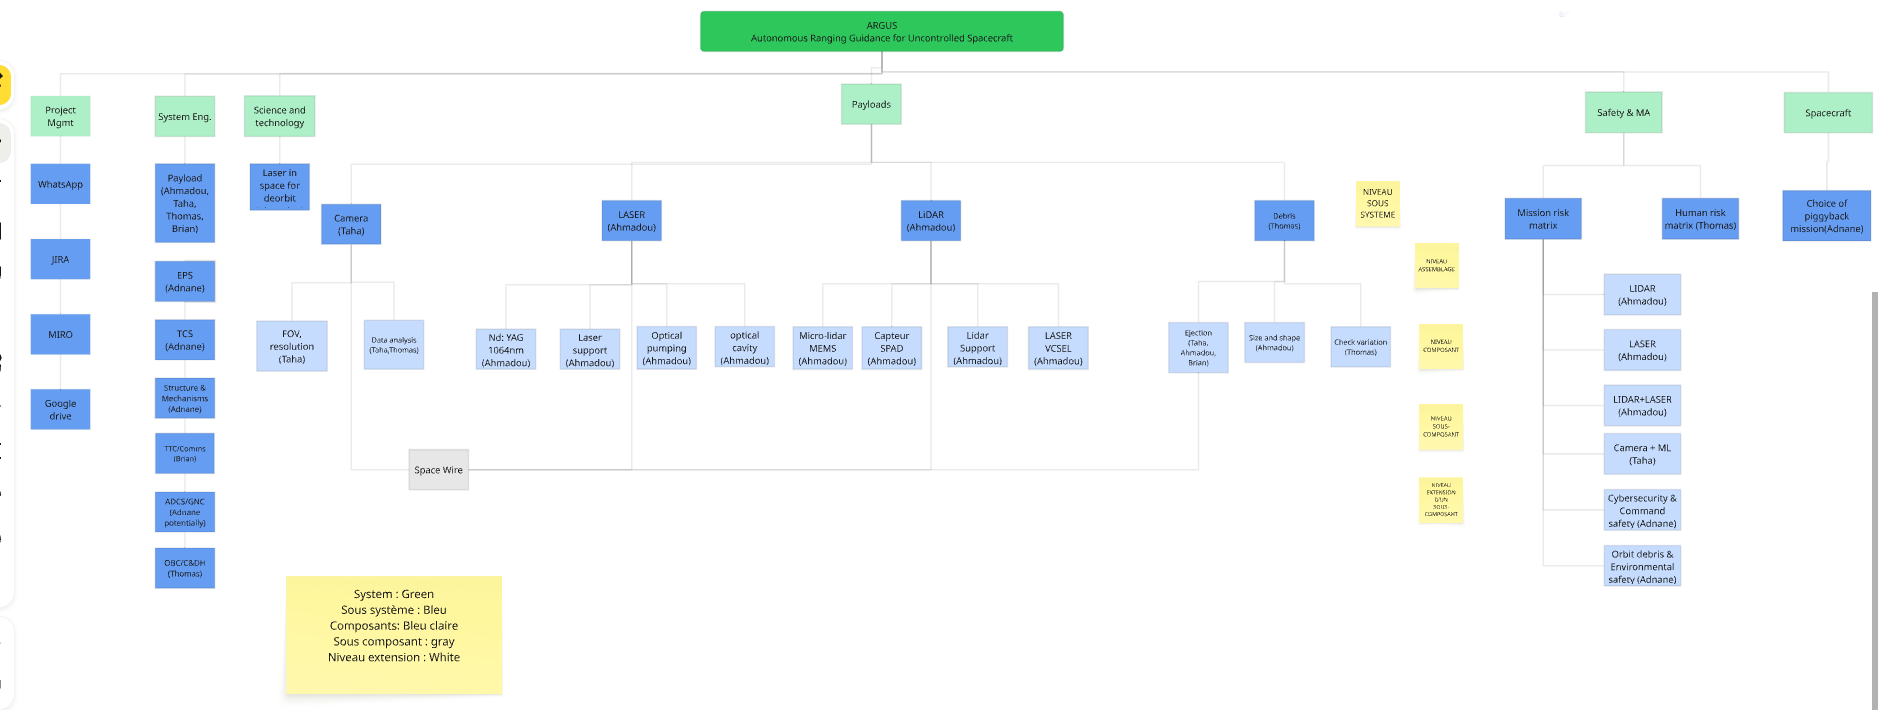
\includegraphics[width=0.8\textwidth]{wbs.png}
    \caption{Work Breakdown Structure.}
    \label{fig:wbs}
\end{figure}

\subsection{Data Management Plan -- functional diagram V1}

\begin{figure}[htbp]
    \centering
    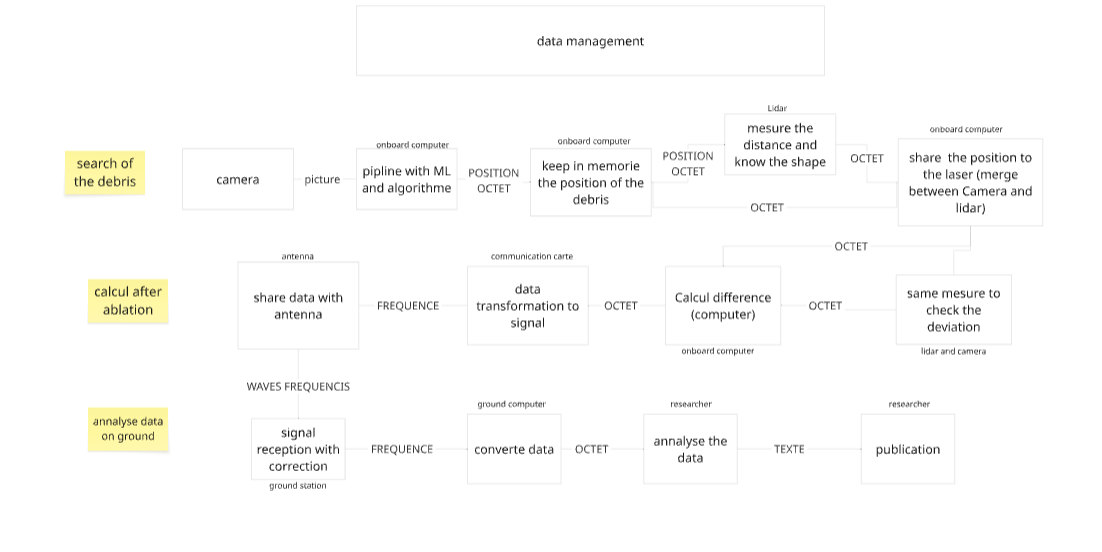
\includegraphics[width=0.8\textwidth]{data_management.png}
    \caption{Data Management Plan -- functional diagram V1.}
    \label{fig:data_management}
\end{figure}

\noindent\textbf{Legend.} The diagram is divided into three phases:
\textit{search of the debris} (detection and localisation),
\textit{calculation after ablation} (check of the laser effect and transmission),
and \textit{analysis of the data on ground}.
Each box is a step of the chain, and the small text next to it gives the equipment
performing the step (onboard computer, lidar, camera, communication board, antenna,
ground station, ground computer, or researcher).
The labels on the arrows give the type of data exchanged:
\textit{picture} (raw camera image),
\textit{position octet} (debris position encoded in bytes),
\textit{octet} (binary data such as measurements and deviation),
\textit{frequency} (radio signal between the antenna and the ground station),
and \textit{text} (final publication).

\subsection{Satellite platform -- functional diagram V1}
\todo{insert the figure look on miro}

\subsection{Satellite system model V1 (IDM-CIC)}

\begin{figure}[htbp]
  \centering
  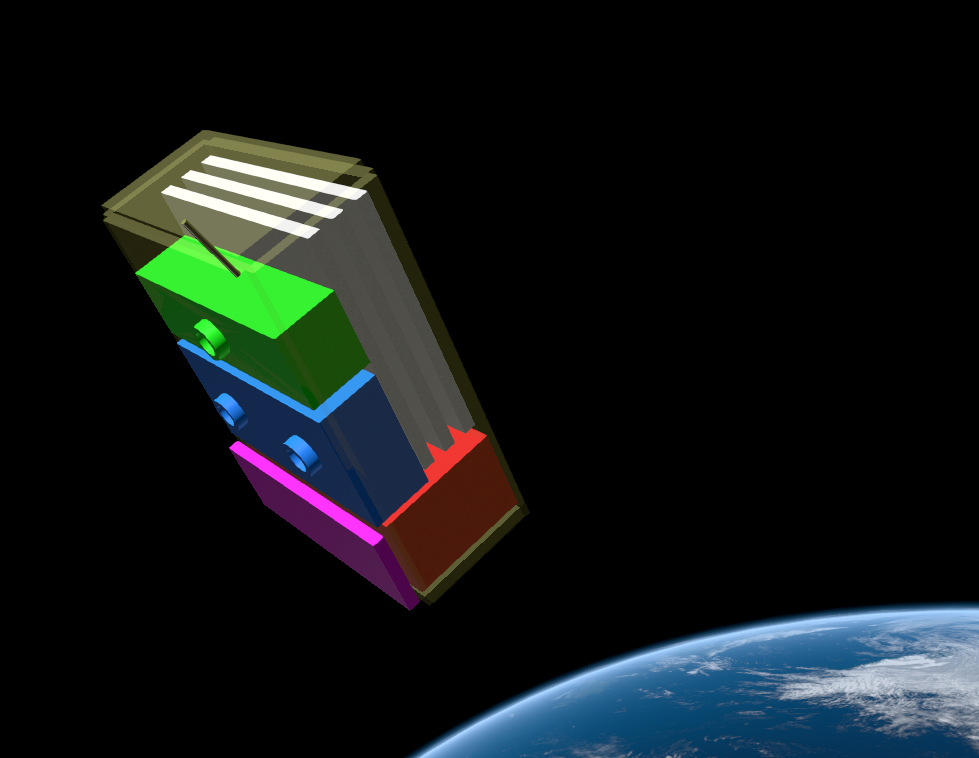
\includegraphics[width=0.8\textwidth]{idmcicv1.png}
  \caption{V1 of the satellite system model (IDM-CIC).}
  \label{fig:idmcicv1}
\end{figure}

Figure~\ref{fig:idmcicv1} shows the internal layout of the Argus satellite. 
The two main payloads are located at the front of the structure. The debris 
payload (purple) sits at the bottom of the payload stack, while the 
class~4 laser (blue) is placed directly above it, with its aperture oriented 
towards the target.

The two secondary payloads are stacked above the main payloads. The LiDAR 
(blue) and the camera (green) are positioned side by side so that their lines 
of sight are aligned with the laser axis. This arrangement allows the camera and 
the LiDAR to detect and track the debris, and to provide the laser with the 
position needed to fire at it. Each of these instruments has a circular opening 
on its front face for its optical aperture.

At the back of the satellite, a stack of thin boards hosts the onboard 
computer and the other subsystems. The battery (red) is located at the bottom 
of the structure, close to the main payloads, which are the most power-demanding 
elements. Finally, the antenna (grey) is mounted at the top of the satellite, 
which allows the data to be sent to the Earth, such as the deviation measured by 
the camera and the LiDAR.
% ==================================================================
\section{Mission Analysis V1}

\todo{orbit and mission phases -- to be discussed with the other subsystem}
\todo{maybe add some seach on procurreezy and vector ifyou have sometjing interresing}

% ==================================================================
\section{Mission Report Summary V1}
\todo{write the summary following the ``Leads for Report Summary''}

% ==================================================================
\section{Risk Analysis}

\subsection{Risks related to the power LASER}

\begin{longtable}{>{\raggedright\arraybackslash}p{3.7cm} >{\raggedright\arraybackslash}p{4.2cm} >{\raggedright\arraybackslash}p{3.7cm} >{\centering\arraybackslash}p{1.4cm} >{\raggedright\arraybackslash}p{4.0cm}}
\risqueentete
Power and heat too high for a 6U & 1\,kW optical with 35\,\% efficiency requires about 2.9\,kW electrical, including nearly 1.9\,kW of heat & Difficult to power and cool the system & High & Reduce $P_{avg}$, favour short shots on battery, perform a thermal study \\
Poor pointing & 3\,mm spot at 50\,m, i.e.\ about 60\,$\mu$rad, very demanding for a CubeSat & Shot misses the debris, no ablation & High & Fine pointing mirror guided by the LiDAR \\
Debris drifts away during firing & With $F = 30$\,mN on 1\,kg, the debris moves away by about 150\,m in 100\,s & Impossible to fire 2433\,s continuously to reach 73\,m/s & High & Short shots, debris tracking, aim for a smaller $\Delta V$ \\
%%Inconsistent sizing values & $E_p$ of 0.35\,J or 0.5\,J, $P_c$ of 70 or 100\,MW, frequency 3000\,Hz (2\,kHz); 0.5\,J $\times$ 3000\,Hz gives 1500\,W, not 1000\,W & Wrong calculations, to be redone & Medium & Fix a single set of values and recalculate everything \\
Ablation efficiency overestimated & $C_m = 30\ \mu$N$\cdot$s/J assumed constant & Lower force and longer firing time & Medium & Take a margin, perform ground tests \\
Damaged optics & 100\,MW peak pulses, aluminium vapour deposition & Power loss, damaged optics & Medium & Margin on damage threshold, protective window \\
Debris fragmentation & Fluence too high or tumbling debris & New debris (Kessler syndrome) & High & Control the fluence, stop firing in case of anomaly \\
Unintended shot or reflection & Highly reflective aluminium surface & Dazzling or damaging another satellite & Medium & Shutter, firing authorized only if the target is locked \\
Hazard to people during tests & Class 4 laser at 1064\,nm & Eye or skin injury & High & Suitable goggles, closed room, laser safety officer \\
Source failure & Ageing of the pump diodes & Loss of the mission & Medium & Operating margin, power monitoring \\
\end{longtable}

\subsection{Risks related to the LiDAR}

\begin{longtable}{>{\raggedright\arraybackslash}p{3.7cm} >{\raggedright\arraybackslash}p{4.2cm} >{\raggedright\arraybackslash}p{3.7cm} >{\centering\arraybackslash}p{1.4cm} >{\raggedright\arraybackslash}p{4.0cm}}
\risqueentete
Millimetre accuracy not reached & 3\,ns pulse and 200\,ps SPAD jitter, i.e.\ about 3\,cm & Position less accurate than expected & Medium & Announce centimetre accuracy, justify millimetre level by averaging \\
Return signal too weak & Small debris, SPAD efficiency of only 20\,\%, aluminium surface & Debris not detected & Medium & Perform a link budget, adjust energy or frequency \\
Sensor dazzling & Ablation laser, plasma, Sun or Earth in the field of view & Blind detection & Medium & 1550\,nm filter, gated operation, shutter \\
Loss of debris tracking & Small tumbling target, field limited to $\pm 10$\textdegree & Firing impossible, target lost & High & Reacquisition algorithm, adapted field of view \\
Sensor degraded by radiation & Increasing dark noise (10\,kHz at start) & False detections & Medium & Cooling, shielding, noise monitoring \\
Fragile MEMS micro-mirror & Vibration effects at launch & Mirror stuck or shifted & Medium & Launch lock, vibration and thermal tests \\
Synchronization and onboard computing & Offset between emission and detection, limited CubeSat computer & Wrong or too slow measurements & Medium & Common clock, lightweight algorithms \\
LiDAR eye safety & 10\,$\mu$J beam at 20\,kHz & Low hazard during tests & Low & Check the standard, limit access \\
\end{longtable}

\subsection{Risks related to the camera and Machine Learning}

\begin{longtable}{>{\raggedright\arraybackslash}p{3.7cm} >{\raggedright\arraybackslash}p{4.2cm} >{\raggedright\arraybackslash}p{3.7cm} >{\centering\arraybackslash}p{1.4cm} >{\raggedright\arraybackslash}p{4.0cm}}
\risqueentete
Missed or false debris detection & Small target, stars or reflections mistaken for debris & Target not acquired or wrong object tracked & High & Train with and without debris, check detection over several images \\
Poor image quality & Shadows, strong reflections or motion blur & Debris features cannot be located reliably & Medium & Adjust exposure, test different lighting conditions, reject unusable images \\
Training images not representative & Mostly simulated images, limited real views of the debris & Good ground results but poor performance in flight & High & Add real images, vary lighting and rotation, keep a separate test set \\
Debris too small in the image & Camera sized for 2--10\,m, target farther away during firing & Detection possible but orientation cannot be estimated & High & Agree on a common operating distance, check target size in pixels \\
Wrong distance or orientation estimate & Symmetric debris, poorly located features or camera calibration error & Incorrect tracking and pointing data & High & Calibrate the camera, check the 3D model, compare distance with the LiDAR \\
Loss of visual tracking & Tumbling debris or target leaving the predicted image region & Position estimate no longer valid, firing interrupted & High & Restart full-image detection, inhibit firing until tracking is confirmed \\
Onboard processing too slow & Two neural networks and tracking running on limited hardware & Two observations per second not reached, delayed pointing data & Medium & Test the complete chain on Q8S and XE2, simplify the models if needed \\
Model deployment failure & Network operations unsupported on XE2 or reduced numerical precision & Model fails to run or gives less accurate results & Medium & Compile both networks early, compare onboard results with ground results \\
Camera and LiDAR data out of sync & Different timestamps, transfer delays or inconsistent reference frames & Measurements refer to different target positions & High & Use a common clock, define reference frames, test the complete sensor interface \\
\end{longtable}

\subsection{Risks related to the whole LiDAR + LASER payload}

\begin{longtable}{>{\raggedright\arraybackslash}p{3.7cm} >{\raggedright\arraybackslash}p{4.2cm} >{\raggedright\arraybackslash}p{3.7cm} >{\centering\arraybackslash}p{1.4cm} >{\raggedright\arraybackslash}p{4.0cm}}
\risqueentete
Payload too heavy or power-hungry for a 6U & Laser, cooling, battery, LiDAR (about 12\,W) and optics to accommodate & Mission not feasible in 6U & High & Mass, volume and power budget with the other teams \\
LiDAR / laser misalignment & Launch vibrations, temperature variations & Laser does not aim where the LiDAR measures & High & Common rigid structure, in-orbit calibration \\
Firing software bug & Error in the logic between detection and firing & Unintended shot or lock-up & High & Simple logic, loop testing \\
Electromagnetic interference & Pulsed laser power supply close to the sensor and the onboard computer & Disturbed measurements, reboots & Medium & Shielding, careful cabling, EMC tests \\
Shocks, vibrations and vacuum & Launch and orbital conditions & Misaligned or broken parts & Medium & Vibration, thermal and vacuum tests \\
Launcher safety requirements & Class 4 laser and battery on board & Integration refused & High & Laser disabled until separation, early dialogue with the launcher \\
Poor debris ejection & Velocity of 0.1 to 0.5\,m/s poorly controlled & Debris returning towards the CubeSat & Medium & Simulate the relative trajectory before flight \\
Loss of communication with the ground & Firing outside the contact windows & Uncontrolled firing & Medium & Firing inhibited by default, safe autonomous sequence \\
Laser cost & Space-qualified 1\,kW pulsed source beyond a student budget & Project blocked & High & Get quotes from suppliers, plan a lower-power demonstrator \\
\end{longtable}



\subsection{Human and organizational risks (related to the subsystem)}

\begin{longtable}{>{\raggedright\arraybackslash}p{3.7cm} >{\raggedright\arraybackslash}p{4.2cm} >{\raggedright\arraybackslash}p{3.7cm} >{\centering\arraybackslash}p{1.4cm} >{\raggedright\arraybackslash}p{4.0cm}}
\risqueentete
%Too many responsibilities on one person & I lead the subsystem alone & Blocked if I am unavailable & Medium & Appoint a deputy, document \\
Unnoticed calculation errors & Different values in different places of the document & Wrong results in the report & Medium & Single calculation file, review by a colleague \\
Limited skills & Little experience in laser, optics and laser safety & Poor technical choices, risk during tests & High & Training, advice from the supervisor or an expert \\
Poor communication between teams & Interfaces with power, thermal, structure and attitude not defined & Incompatibilities discovered too late & Medium & Regular meetings, interface document \\
Optimism on assumptions & Values chosen so that the calculation works (1\,kW, 73\,m/s) & Reality may be different & Medium & External review, explicit margins \\
%Incomplete references & ``ref to add'' and ``to complete'' in the document & Questionable sources & Low & Complete all references \\
Handling error during tests & Laser or high voltage without protocol & Personal injury & High & Written protocol, work in pairs, emergency stop \\
\end{longtable}

\subsection{Risk analysis for the participants}

Probability / severity, each rated out of 5 (5 = maximum).

\begin{longtable}{>{\raggedright\arraybackslash}p{5.6cm} >{\centering\arraybackslash}p{2.6cm} >{\raggedright\arraybackslash}p{8.8cm}}
\toprule
\textbf{Problem} & \textbf{Prob. / Severity} & \textbf{Solution} \\
\midrule
\endfirsthead
\toprule
\textbf{Problem} & \textbf{Prob. / Severity} & \textbf{Solution} \\
\midrule
\endhead
\bottomrule
\endfoot
Loss or breakage of a computer & 2/4 & Backup device, handwriting \\
Long-term illness & 3/2 & Share the work, work more after recovery \\
Inability to work & 2/5 & Scale the project down, increase each person's workload \\
Exclusion from the master's programme & 1/5 & Same as above \\
Work overload (other courses, exams, internship) & 3/4 & Rely on a good schedule \\
Incompatible availabilities between members & 4/3 & Video meetings and/or state availabilities in advance, read the meeting minutes afterwards \\
Poor workload estimation & 3/3 & Redistribute the work among us, report it in a meeting or to the coordinator \\
Working on the same parts & 4/4 & Define the tasks with the WBS \\
Timing problem for deliverables & 3/5 & Respect the milestones set at the beginning of the year \\
\end{longtable}



\end{document}